\section{Reading Motion Graphs}
\label{sec:graphs}

Everything in this chapter has come in threes: position, velocity, acceleration; $\tfrac12 a t^2$, $at$, $a$; a curve, a line, a constant. This section puts the three side by side as \emph{graphs} of a single motion and shows how to read any one of them from the others. Section~\ref{sec:calculus} already gave the rules: going \emph{down} the list, from position to velocity to acceleration, you take a slope; going \emph{up} you take an area. What remains is practice at seeing those rules on paper. A motion graph is the commonest form in which information about motion reaches you, whether from a lab cart, a car's data recorder, or a satellite, and reading one fluently is a skill worth a few pages.

\subsection{Three graphs of one motion}

Figure~\ref{fig:threegraphs} shows a cart on a straight track. It starts from rest, speeds up steadily for two seconds, coasts at constant velocity for three seconds, then brakes steadily to a stop in two more. The three graphs are stacked so that the same instant lies on the same vertical line in all three, and the dashed lines at $t = \SI{2}{\second}$ and $t = \SI{5}{\second}$ mark where the motion changes character. Read the figure from the bottom up and from the top down.

\emph{From the bottom up: areas.} The acceleration--time graph is three horizontal steps: $+\SI{1.0}{\metre\per\second\squared}$, then zero, then $\SI{-1.0}{\metre\per\second\squared}$. The area under it over any interval is the change in velocity over that interval (Equation~\eqref{eq:ftc}). The first step encloses a rectangle of area $\SI{1.0}{\metre\per\second\squared} \times \SI{2}{\second} = \SI{2.0}{\metre\per\second}$, so the velocity rises from $0$ to \SI{2.0}{\metre\per\second} by $t = \SI{2}{\second}$; the middle step encloses no area, so the velocity stays put; the last step encloses an area of $\SI{-2.0}{\metre\per\second}$, which brings the velocity back to zero. That is exactly the velocity--time graph in the middle panel: a rising line, a flat line, a falling line. The area under \emph{that} graph, in turn, is the displacement. The shaded triangle under the rising line has area $\tfrac12 \times \SI{2}{\second} \times \SI{2.0}{\metre\per\second} = \SI{2.0}{\metre}$, so the cart is at $x = \SI{2.0}{\metre}$ after two seconds, which is where the position--time graph at the top puts it.

\emph{From the top down: slopes.} The position--time graph is a curve that bends upward, then a straight line, then a curve that flattens out. Its slope at any instant is the velocity. On the first piece the slope starts at zero and grows: the cart is speeding up. On the straight piece the slope is constant: the cart coasts. On the last piece the slope shrinks to zero: the cart is braking to rest. Those slopes, plotted against time, are the middle panel. The slope of the middle panel is in turn the acceleration, and its three constant slopes are the three steps of the bottom panel.

\begin{figure}[htbp]
\centering
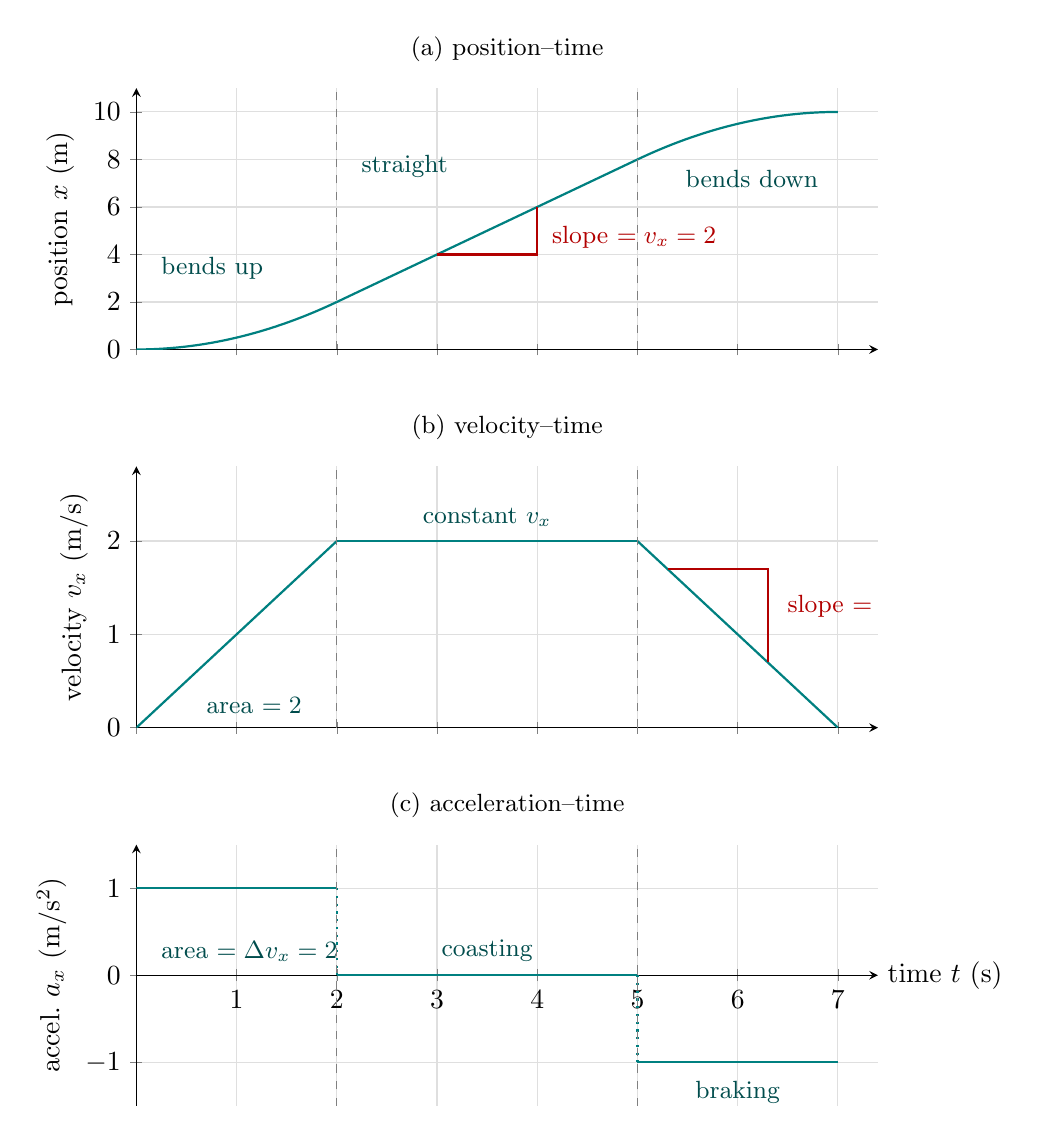
\begin{tikzpicture}
\begin{axis}[
  name=xt,
  width=11cm,height=4.9cm,
  ylabel={position $x$ (m)},
  xmin=0,xmax=7.4,ymin=0,ymax=11,
  xtick={0,1,...,7},ytick={0,2,4,6,8,10},
  grid=major,grid style={gray!25},
  axis lines=left,
  xticklabels={},
  title={(a) position--time},title style={font=\small},
]
\addplot[teal,thick,domain=0:2,samples=30] {0.5*x^2};
\addplot[teal,thick,domain=2:5,samples=2] {2+2*(x-2)};
\addplot[teal,thick,domain=5:7,samples=30] {8+2*(x-5)-0.5*(x-5)^2};
\draw[dashed,gray] (axis cs:2,0) -- (axis cs:2,11);
\draw[dashed,gray] (axis cs:5,0) -- (axis cs:5,11);
\draw[red!70!black,thick] (axis cs:3,4) -- (axis cs:4,4) -- (axis cs:4,6);
\node[red!70!black,font=\small,anchor=north west] at (axis cs:4.05,5.6) {slope $= v_x = \SI{2}{\metre\per\second}$};
\node[teal!60!black,font=\small,anchor=west] at (axis cs:0.15,3.4) {bends up};
\node[teal!60!black,font=\small,anchor=east] at (axis cs:6.9,7.2) {bends down};
\node[teal!60!black,font=\small,anchor=north west,align=left] at (axis cs:2.15,8.6) {straight};
\end{axis}
\begin{axis}[
  name=vt,
  at={(xt.below south west)},anchor=above north west,yshift=-4mm,
  width=11cm,height=4.9cm,
  ylabel={velocity $v_x$ (m/s)},
  xmin=0,xmax=7.4,ymin=0,ymax=2.8,
  xtick={0,1,...,7},ytick={0,1,2},
  grid=major,grid style={gray!25},
  axis lines=left,
  xticklabels={},
  title={(b) velocity--time},title style={font=\small},
]
\addplot[teal!25,draw=none] coordinates {(0,0) (2,2) (2,0)} \closedcycle;
\addplot[teal,thick,domain=0:2,samples=2] {x};
\addplot[teal,thick,domain=2:5,samples=2] {2};
\addplot[teal,thick,domain=5:7,samples=2] {7-x};
\draw[dashed,gray] (axis cs:2,0) -- (axis cs:2,2.8);
\draw[dashed,gray] (axis cs:5,0) -- (axis cs:5,2.8);
\node[teal!60!black,font=\small,anchor=south west] at (axis cs:0.6,0.05) {area $= \SI{2}{\metre}$};
\draw[red!70!black,thick] (axis cs:5.3,1.7) -- (axis cs:6.3,1.7) -- (axis cs:6.3,0.7);
\node[red!70!black,font=\small,anchor=west] at (axis cs:6.4,1.3) {slope $= a_x$};
\node[teal!60!black,font=\small,anchor=south] at (axis cs:3.5,2.05) {constant $v_x$};
\end{axis}
\begin{axis}[
  name=at,
  at={(vt.below south west)},anchor=above north west,yshift=-4mm,
  width=11cm,height=4.9cm,
  xlabel={time $t$ (s)},ylabel={accel.\ $a_x$ (m/s$^2$)},
  xmin=0,xmax=7.4,ymin=-1.5,ymax=1.5,
  xtick={0,1,...,7},ytick={-1,0,1},
  grid=major,grid style={gray!25},
  axis x line=middle,axis y line=left,
  xlabel style={at={(axis description cs:1,0.5)},anchor=west},
  title={(c) acceleration--time},title style={font=\small},
]
\addplot[teal!25,draw=none] coordinates {(0,0) (0,1) (2,1) (2,0)} \closedcycle;
\addplot[teal,thick,domain=0:2,samples=2] {1};
\addplot[teal,thick,domain=2:5,samples=2] {0};
\addplot[teal,thick,domain=5:7,samples=2] {-1};
\draw[teal,thick,dotted] (axis cs:2,1) -- (axis cs:2,0);
\draw[teal,thick,dotted] (axis cs:5,0) -- (axis cs:5,-1);
\draw[dashed,gray] (axis cs:2,-1.5) -- (axis cs:2,1.5);
\draw[dashed,gray] (axis cs:5,-1.5) -- (axis cs:5,1.5);
\node[teal!60!black,font=\small,anchor=south west] at (axis cs:0.15,0.05) {area $= \Delta v_x = \SI{2}{\metre\per\second}$};
\node[teal!60!black,font=\small,anchor=north] at (axis cs:6,-1.1) {braking};
\node[teal!60!black,font=\small,anchor=south] at (axis cs:3.5,0.05) {coasting};
\end{axis}
\end{tikzpicture}
\caption{Three graphs of one motion: a cart that speeds up at \SI{1.0}{\metre\per\second\squared} for \SI{2}{\second}, coasts at \SI{2.0}{\metre\per\second} for \SI{3}{\second}, then brakes at \SI{1.0}{\metre\per\second\squared} to a stop at $t = \SI{7}{\second}$. The same instant lies on the same vertical line in all three panels. Going down the stack, each graph is the slope of the one above: the velocity in (b) is the slope of (a), and the acceleration in (c) is the slope of (b). Going up, each graph is the area under the one below: the shaded triangle in (b) is the cart's displacement in the first two seconds, and the shaded rectangle in (c) is its gain in velocity over the same interval. The velocity--time graph has corners where the acceleration jumps; the position--time graph has none, because the velocity never jumps.}
\label{fig:threegraphs}
\end{figure}

\begin{keyidea}[How to read the three graphs]
\begin{center}
\renewcommand{\arraystretch}{1.4}
\small
\begin{tabular}{llll}
\toprule
graph & its height is & its slope is & the area under it is \\
\midrule
position--time & position $x$ & velocity $v_x$ & (nothing useful) \\
velocity--time & velocity $v_x$ & acceleration $a_x$ & displacement $\Delta x$ \\
acceleration--time & acceleration $a_x$ & (rarely needed) & change in velocity $\Delta v_x$ \\
\bottomrule
\end{tabular}
\end{center}
\elemtag\ Slope means rise over run, estimated with a ruler laid along the curve; area means the geometry of rectangles, triangles, and trapezia, counted negative below the time axis. \calctag\ Slope means the derivative and area means the definite integral; the two rows of Equation~\eqref{eq:ftc} are the last column of the table. A \emph{straight} position--time graph means constant velocity and zero acceleration. A \emph{curved} one means the velocity is changing: if the curve bends upward (holds water) the slope is increasing and $a_x > 0$; if it bends downward (spills water) the slope is decreasing and $a_x < 0$. \calctag\ Which way the curve bends is the sign of $\dd^2 x/\dd t^2$, which is $a_x$.
\end{keyidea}

Two cautions before the examples. First, none of these graphs is a picture of the cart's path. The cart moves along a straight track; the position--time graph goes up and around because its \emph{vertical} axis is position and its horizontal axis is time. A ball thrown straight up has a position--time graph shaped like an arch (Exercise~\ref{ex:graphtruth}), but its path is a vertical line. Second, the sign of the velocity and the sign of the acceleration are read from different graphs and can disagree. A velocity--time graph that is positive but falling describes an object moving forward and slowing down; one that is negative and falling describes an object moving backward and speeding up. In both cases $a_x < 0$. ``Slowing down'' is not what a negative acceleration means; it means the velocity is decreasing, which is the same thing only when the velocity is positive.

\begin{example}{Reading a trip from its graphs}{graphtrip}
Use Figure~\ref{fig:threegraphs} to find (a) the cart's acceleration in each of the three phases, (b) its displacement in each phase and in total, and (c) its position at $t = \SI{6}{\second}$. Then (d) say why the velocity--time graph has corners but the position--time graph does not.

\elem (a) Acceleration is the slope of the velocity--time graph. From $t = 0$ to \SI{2}{\second} the velocity rises by \SI{2.0}{\metre\per\second} in \SI{2}{\second}: slope $+\SI{1.0}{\metre\per\second\squared}$. From \SI{2}{\second} to \SI{5}{\second} the graph is flat: slope $0$. From \SI{5}{\second} to \SI{7}{\second} it falls by \SI{2.0}{\metre\per\second} in \SI{2}{\second}: slope $\SI{-1.0}{\metre\per\second\squared}$. These are the three steps of panel (c).

(b) Displacement is the area under the velocity--time graph. Phase one is a triangle: $\tfrac12 (2)(2.0) = \SI{2.0}{\metre}$. Phase two is a rectangle: $(3)(2.0) = \SI{6.0}{\metre}$. Phase three is another triangle: $\tfrac12 (2)(2.0) = \SI{2.0}{\metre}$. Total: \SI{10}{\metre}, which is where panel (a) ends. Equivalently, the whole graph is a trapezium with parallel sides \SI{7}{\second} and \SI{3}{\second} and height \SI{2.0}{\metre\per\second}: $\tfrac12(7 + 3)(2.0) = \SI{10}{\metre}$.

(c) At $t = \SI{6}{\second}$ the cart is one second into the braking phase. Its velocity has dropped from \SI{2.0}{\metre\per\second} to \SI{1.0}{\metre\per\second}, so its average velocity over that second was \SI{1.5}{\metre\per\second} and it moved \SI{1.5}{\metre}. It was at \SI{8.0}{\metre} at $t = \SI{5}{\second}$, so it is at \SI{9.5}{\metre}. Reading panel (a) directly gives the same value.

\calc (a) Write the velocity piecewise from panel (b): $v_x = t$ for $0 \le t \le 2$, $v_x = 2$ for $2 \le t \le 5$, and $v_x = 7 - t$ for $5 \le t \le 7$ (SI units). Differentiating each piece gives $a_x = 1, 0, -1$ in \si{\metre\per\second\squared}.

(b) Integrate each piece: $\int_0^2 t\,\dd t = 2$, $\int_2^5 2\,\dd t = 6$, $\int_5^7 (7 - t)\,\dd t = [7t - \tfrac12 t^2]_5^7 = 24.5 - 22.5 = 2$; total \SI{10}{\metre}. Integrating once more with $x(0) = 0$ gives the position piecewise, $x = \tfrac12 t^2$, then $x = 2 + 2(t - 2)$, then $x = 8 + 2(t - 5) - \tfrac12 (t - 5)^2$, which is the curve plotted in panel (a).

(c) $x(6) = 8 + 2(1) - \tfrac12(1)^2 = \SI{9.5}{\metre}$.

(d) A corner on a graph is a place where the slope jumps. The slope of the velocity--time graph is the acceleration, and the acceleration does jump, from $+1$ to $0$ at $t = \SI{2}{\second}$ and from $0$ to $-1$ at $t = \SI{5}{\second}$; so the velocity--time graph has corners there. The slope of the position--time graph is the velocity, and the velocity changes \emph{continuously}, since a finite acceleration cannot change it by a finite amount in no time at all. So the position--time graph is smooth: the parabola, the line, and the second parabola join with matching slopes, \SI{2.0}{\metre\per\second} at both joins.\qed
\end{example}

\begin{modelnote}[Steps and corners]
The acceleration--time graph in Figure~\ref{fig:threegraphs} jumps instantly from one value to another, and the velocity--time graph has sharp corners. Both are idealisations. A real motor takes a fraction of a second to reach full thrust, and real brakes take a fraction of a second to bite, so a real acceleration--time graph has short ramps in place of the vertical jumps and the real velocity--time graph has rounded corners. On a graph spanning seven seconds the rounding is too small to draw, and the step model captures everything that matters for the displacement. The lesson generalises: a position--time graph is always smooth, a velocity--time graph can have corners, and an acceleration--time graph can have jumps, because each is one derivative rougher than the one above it.
\end{modelnote}

\begin{example}{From a position--time graph downward}{xtgraph}
A cart's position--time graph is the parabola $x = 4t - t^2$ (metres, $t$ in seconds) for $0 \le t \le \SI{4}{\second}$. Reading the graph rather than the formula wherever you can: (a) When is the cart momentarily at rest, and where is it then? (b) Is the acceleration positive or negative, and what is its value? (c) What are the cart's displacement and its distance travelled over the four seconds? (d) Sketch the velocity--time and acceleration--time graphs.

\elem (a) The graph rises, levels off, and falls: an arch. The cart is at rest where the tangent is horizontal, at the top of the arch. The parabola is symmetric, crossing $x = 0$ at $t = 0$ and $t = \SI{4}{\second}$, so its top is at $t = \SI{2}{\second}$, where $x = 8 - 4 = \SI{4}{\metre}$.

(b) The arch bends downward, so the slope is decreasing throughout and the acceleration is negative. For its value, read positions at whole seconds, $x = 0, 3, 4, 3, 0$, and take first differences: $+3, +1, -1, -3$~m in successive seconds. These are the average velocities, and they drop by \SI{2}{\metre\per\second} every second: $a_x = \SI{-2}{\metre\per\second\squared}$. (The second differences are all $-2$, the odd-number rule running in reverse.)

(c) The displacement is the change in the graph's height: $x(4) - x(0) = 0$. The cart ends where it began. The distance travelled is not zero: it went \SI{4}{\metre} out to the top of the arch and \SI{4}{\metre} back, \SI{8}{\metre} in all. A position--time graph shows displacement at a glance and distance only if you add up the ups and downs separately.

(d) The velocity--time graph is the slope of the arch: a straight line falling steadily, starting at $+\SI{4}{\metre\per\second}$, crossing zero at $t = \SI{2}{\second}$, and ending at $\SI{-4}{\metre\per\second}$. Its slope is $-2$, so the acceleration--time graph is a horizontal line at $\SI{-2}{\metre\per\second\squared}$. As a check, the velocity--time line encloses a triangle of area $+4$ above the axis and a triangle of area $-4$ below it, total zero, which is the displacement found in (c).

\calc (a) $v_x = \dd x/\dd t = 4 - 2t$, zero at $t = \SI{2}{\second}$, where $x = \SI{4}{\metre}$. (b) $a_x = \dd v_x/\dd t = -2$: negative, and constant. (c) $\Delta x = \int_0^4 (4 - 2t)\,\dd t = 16 - 16 = 0$; distance $= \int_0^4 |4 - 2t|\,\dd t = 2\int_0^2 (4 - 2t)\,\dd t = \SI{8}{\metre}$. (d) $v_x = 4 - 2t$ is a line of slope $-2$; $a_x = -2$ is a horizontal line.

This is the thrown ball of Figure~\ref{fig:thrown} in miniature, with $v_0 = \SI{4}{\metre\per\second}$ and $g$ replaced by \SI{2}{\metre\per\second\squared}: same arch, same straight velocity line through zero at the top, same constant negative acceleration. Every constant-acceleration motion produces this trio of shapes.\qed
\end{example}

\begin{checkbox}
Figure~\ref{fig:thrown} is the velocity--time graph of a ball thrown straight up at \SI{15}{\metre\per\second}. Sketch the matching position--time and acceleration--time graphs. What does the position--time graph look like at the top of the flight? What is the area under the acceleration--time graph between $t = 0$ and $t = \SI{3.06}{\second}$, and what does that area represent?
\end{checkbox}

